% Reformat of Document Version 1.0.1: 29 August 2000
% Document Version 1.0.1: 29 August 2000

\documentclass{report}


\usepackage{geometry}
\geometry{letterpaper, portrait, margin=0.75in}
\usepackage{pdfpages}
\usepackage{color}
\usepackage{soul}
\usepackage{parskip}
\usepackage{multicol}
\usepackage[T1]{fontenc}
\usepackage{ascii}

% \usepackage{newtxtt}
%\makeatletter
%\renewcommand{\verbatim@font}{\usefont{T1}{newtxtt}{m}{n}}
%\makeatother

% need to use xelatex or lualatex for fontspec

% Adding this to override usual mono spaced font for 'verbatim' environment
% Doing this because original document uses courier mono for a specific purpose
% I usually use verbatim as crutch to get something with weird symbols to work right.

\usepackage{fontspec}
\setmainfont{DejaVu Serif}
\setsansfont{DejaVu Sans}
\setmonofont{DejaVu Sans Mono}
% \makeatletter

\newcommand{\setverbatimfont}[1]{\def\m@mverbfont{#1}}
\setverbatimfont{DejaVu Sans}
% \usepackage{AnonymousPro}
% \newfontfamily\TypeWriterFont[ttdefault=true]{AnonymousPro}
\newcommand{\TypeWriterFont}[0]{\texttt}

\title{AUTOMATIC POSITION REPORTING SYSTEM}
\date{29 August 2000}
\author{The APRS Working Group}

\begin{document}

\maketitle



 \part*{Document Covers}

\section*{Cover One}

% Put cover page from PDF here.
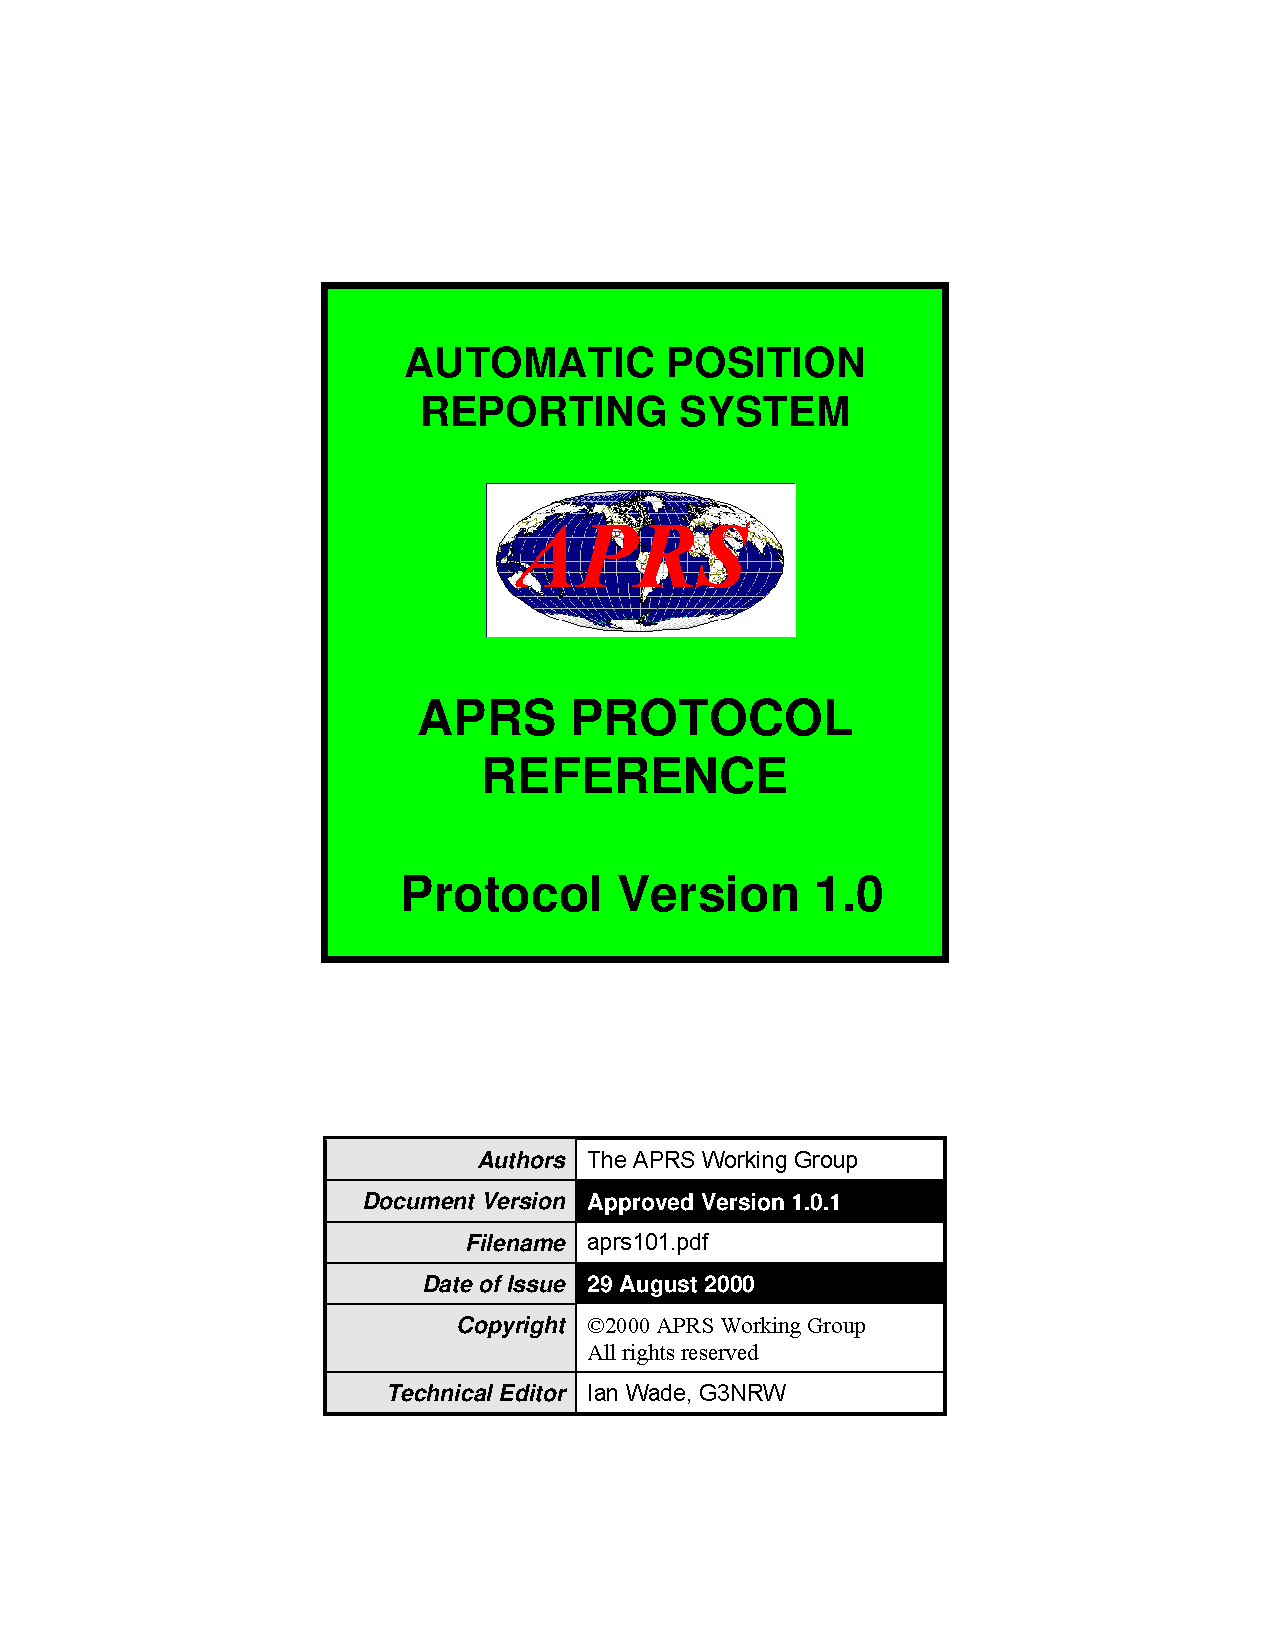
\includepdf[pages=1] {APRS101-original.pdf}

\section*{Cover Two}

\begin{verbatim}
AUTOMATIC POSITION REPORTING SYSTEM

APRS PROTOCOL REFERENCE
Protocol Version 1.0

Authors The APRS Working Group
Document Version Approved Version 1.0.1
Filename aprs101.pdf
Date of Issue 29 August 2000
Copyright ©2000 APRS Working Group
All rights reserved
Technical Editor Ian Wade, G3NRW
\end{verbatim}

\newpage

\section*{Cover Three}

\begin{verbatim}
APRS Protocol Reference
Protocol Version 1.0
by the APRS Working Group
Edited by Ian Wade

Published by
Tucson Amateur Packet Radio Corp
8987–309 East Tanque Verde Road, #337
Tucson, AZ 85749-9399
United States of America
http://www.tapr.org
ISBN 0-9644707-6-4
TAPR Publication Number: 99-4

Copyright ©2000 APRS Working Group
All rights reserved

APRS® is a registered trademark of Bob Bruninga.
WinAPRS™, MacAPRS™, X-APRS™, PalmAPRS™ and APRS/CE™
are trademarks using the APRS® name, licensed from Bob Bruninga.
This document may be copied for non-commercial purposes only, and must
include the above copyright statement and trademark statements in full.
\end{verbatim}

\newpage
\section*{Cover Four: Note on Reformatted Version}
To be added





% Part 0 Chunk 1

 % Prelude Part One

\part*{Prelude}

\section*{FOREWORD}

This APRS Protocol Reference document represents the coming-of-age of WB4APR’s baby.
Starting with a simple concept — a way to track the location of moving objects via packet radio
— programs using the APRS protocol have grown into perhaps the most popular packet radio
application in use today. It’s also become one of the most complex; from the simple idea grew,
and still grows, a tactical communications system of tremendous capability. Like many ham
projects, the APRS protocol was designed as it was being implemented, and many of its
intricacies have never been documented.

Until now. This specification defines the APRS on-air protocol with a precision and clarity that
make it a model for future efforts. The work done by members of the APRS Working Group, as
well as Technical Editor Ian Wade, G3NRW, should be recognized as a tremendous contribution
to the packet radio art. With this document available, there is now no excuse for any developer to
improperly implement the APRS protocol.

As an APRS Working Group member whose role was mainly that of observer, I was fascinated
with the interplay among the APRS authors and the Technical Editor as the specification took
form. Putting onto paper details that previously existed only in the minds of the authors exposed
ambiguities, unconsidered consequences, and even errors in what the authors thought they knew.
The discussion that followed each draft, and the questions Ian posed as he tried to wring out the
uncertainties, gave everyone a better understanding of the protocol. I am sure that this process has
already contributed to better interoperability among existing APRS applications.
Everyone who has watched the specification develop, from the initial mention in April 1999 until
release of this Version 1.0 document in August 2000, knows that the process took much longer
than was hoped. At the same time, they saw the draft transformed from a skeleton into a hefty
book of over 110 pages. With the specification now in hand, I think we can all say the wait was
worth it. Congratulations to the APRS Working Group and, in particular, to G3NRW, for a major
contribution to the literature of packet radio.

\begin{verbatim}
John Ackermann, N8UR
TAPR Vice President and APRS Working Group Administrative Chair
August 2000
\end{verbatim}


% TOC to follow


 \tableofcontents

% Part 0 Chunk 2

 \section*{Preamble}

\subsection*{APRS Working Group}

The APRS Working Group is an unincorporated association whose members
undertake to further the use and enhance the value of the APRS protocols by
(a) publishing and maintaining a formal APRS Protocol Specification; (b)
publishing validation tests and other tools to enable compliance with the
Specification; (c) supporting an APRS Certification program; and (d) generally
working to improve the capabilities of APRS within the amateur radio
community.

Although the Working Group may receive support from TAPR and other
organizations, it is an independent body and is not affiliated with any
organization. The Group has no budget, collects no dues, and owns no assets.
The current members of the APRS Working Group are:

\begin{itemize}
\item John Ackermann, N8UR Administrative Chair \& TAPR Representative
\item Bob Bruninga, WB4APR Technical Chair, founder of APRS
\item Brent Hildebrand, KH2Z Author of APRS+SA
\item Stan Horzepa, WA1LOU Secretary
\item Mike Musick, N0QBF Author of pocketAPRS
\item Keith Sproul, WU2Z Co-Author of WinAPRS/MacAPRS/X-APRS
\item Mark Sproul, KB2ICI Co-Author of WinAPRS/MacAPRS/X-APRS
\end{itemize}

\section*{Acknowledgements}
This document is the result of contributions from many people. It includes
much of the material produced by individual members of the Working
Group.

In addition, the paper on the Mic-E data format by Alan Crosswell, N2YGK,
and Ron Parsons, W5RKN was a useful starting point for explaining the
complications of this format.

\section*{Document Version Number}

Except for the very first public draft release of the APRS Protocol
Reference, the document version number is a 3-part number “P.p.D” (for
an approved document release) or a 4-part number “P.p.Dd” (for a draft
release):


% Figure/Table  Here


Thus, for example:

\begin{itemize}

\item Document version number “1.2.3” refers to document release 3 covering
APRS Protocol Version 1.2.

\item Document version number “1.2.3c” is draft “c” of that document.

\end{itemize}


\section*{Release History}

The release history for this document is listed in Appendix 7.

\section*{Document Conventions}

This document uses the following conventions:
\begin{itemize}

\item \texttt {Courier font} ASCII characters in APRS data.

\item \textvisiblespace  ASCII space character.

\item … (ellipsis) zero or more characters.

\item /\$ Symbol from Primary Symbol Table.

\item \textbackslash\$ Symbol from Alternate Symbol Table.

\item 0x hexadecimal (e.g. 0x1d).

\item All callsigns are assumed to have SSID –0 unless otherwise specified.

\item \hl{Yellow marker} (appears as light gray background in hard copy).
Marks text of interest — especially useful for highlighting single
literal ASCII characters (e.g. ") where they appear in APRS data.

\item Shaded areas in packet format diagrams are optional fields.

\end{itemize}

\section*{Feedback}

Please address your feedback or other comments regarding this document to
the TAPR aprsspec mail list.

To join the list, start at http://www.tapr.org and then follow the path Special
Interest Groups $\Rightarrow$ APRS Specification $\Rightarrow$ Join APRS Spec Discussion List.


\section*{Authors’ Foreword}

This reference document describes what is known as APRS Protocol
Version 1.0, and is essentially a description of how APRS operates
today.  It is intended primarily for the programmer who wishes to
develop APRS compliant applications, but will also be of interest to
the ordinary user who wants to know more about what goes on “under the
hood”.  It is not intended, however, to be a dry-as-dust, pedantic,
RFC-style programming specification, to be read and understood only by
the Mr Spocks of this world. We have included many items of general
information which, although strictly not part of the formal protocol
description, provide a useful background on how APRS is actually used
on the air, and how it is implemented in APRS software. We hope this
will put APRS into perspective, will make the document more readable,
and will not offend the purists too much.

It is important to realize how APRS originated, and to understand the
design philosophy behind it. In particular, we feel strongly that APRS
is, and should remain, a light-weight tactical system — almost anyone
should be able to use it in temporary situations (such as emergencies
or mobile work or weather watching) with the minimum of training and
equipment.

This document is the result of inputs from many people, and collated
and massaged by the APRS Working Group. Our sincere thanks go to
everyone who has contributed in putting it together and getting it
onto the street. If you discover any errors or omissions or misleading
statements, please let us know — the best way to do this is via the
TAPR aprsspec mailing list at www.tapr.org.

Finally, users throughout the world are continually coming up with new
ideas and suggestions for extending and improving APRS. We welcome
them.  Again, the best way to discuss these is via the aprsspec list.

--The APRS Working Group, August 2000


\section*{Disclaimer}

Like any navigation system, APRS is not infallible. No one should rely
blindly on APRS for navigation, or in life-and-death situations. Similarly,
this specification is not infallible.

The members of the APRS Working Group have done their best to define the
APRS protocol, but this protocol description may contain errors, or there
may be omissions. It is very likely that not all APRS implementations will
fully or correctly implement this specification, either today or in the future.


We urge anyone using or writing a program that implements this
specification to exercise caution and good judgement. The APRS Working
Group and the specification’s Editor disclaim all liability for injury to
persons or property that may result from the use of this specification or
software implementing it.



% Part 1 Chapter 0

 \part{The Structure of this Specification}

This specification describes the overall requirements for developing software
that complies with APRS Protocol Version 1.0. The information flow starts
with the standard AX.25 UI-frame, and progresses downwards into more and
more detail as the use of each field in the frame is explored.
A key feature of the specification is the inclusion of dozens of detailed
examples of typical APRS packets and related math computations.
Here is an outline of the chapters:

% reduce baseline skip for this section

\paragraph{Introduction to APRS --}A brief background to APRS and a summary of its
main features.

\paragraph{The APRS Design Philosophy --}The fundamentals of APRS, highlighting
its use as a real-time tactical communications tool, the timing of
APRS transmissions and the use of generic digipeating.

\paragraph{APRS and AX.25 --}A brief refresher on the structure of the AX.25
UI-frame, with particular reference to the special ways in which APRS uses
the Destination and Source Address fields and the Information field.

\paragraph{APRS Data in the AX.25 Destination and Source Address Fields --}
Details of generic APRS callsigns and callsigns that specify display symbols
and APRS software version numbers. Also a summary of how Mic-E
encoded data is stored in the Destination Address field, and how the Source
Address SSID can specify a display icon.

\paragraph{APRS Data in the AX.25 Information Field --}Details of the principal
constituents of APRS data that are stored in the Information field. Contains
the APRS Data Type Identifiers table, and a summary of all the different
types of data that the Information field can hold.

\paragraph{Time and Position Formats --}Information on formats for timestamps,
latitude, longitude, position ambiguity, Maidenhead locators, NMEA data
and altitude.

\paragraph{APRS Data Extensions --}Details of optional data extensions for station
course/speed, wind speed/direction, power/height/gain, pre-calculated radio
range, DF signal strength and Area Object descriptor.

\paragraph{Position and DF Report Data Formats --}Full details of these report
formats.

\paragraph{Compressed Position Report Data Formats --}Full details of how station
position and APRS data extensions are compressed into very short packets.

\paragraph{Mic-E Data Format --}Mic-E encoding of station lat/long position, altitude,
course, speed, Mic-E message code, telemetry data and APRS digipeater
path into the AX.25 Destination Address and Information fields.

\paragraph{Object and Item Reports --}Full information on how to set up APRS
Objects and Items, and details of the encoding of Area Objects (circles, lines,
ellipses etc).

\paragraph{Weather Reports --}Full format details for weather reports from
standalone (positionless) weather stations and for reports containing
position information. Also details of storm data format.

\paragraph{Telemetry Data --}A description of the MIM/KPC-3+ telemetry data
format, with supporting information on how to tailor the interpretation of the
raw data to individual circumstances.

\paragraph{Messages, Bulletins and Announcements --}Full format information.

\paragraph{Station Capabilities, Queries and Responses --}Details of the ten different
types of query and expected responses.

\paragraph{Status Reports --}The format of general status messages, plus the special
cases of using a status report to contain meteor scatter beam heading/power
and Maidenhead locator.

\paragraph{Network Tunneling --}The use of the Source Path Header to allow
tunneling of APRS packets through third-party networks that do not
understand AX.25 addresses, and the use of the third-party Data Type
Identifier.

\paragraph{User-Defined Data Format --}APRS allows users to define their own data
formats for special purposes. This chapter describes how to do this.

\paragraph{Other Packets --} A general statement on how APRS is to handle any other
packet types that are not covered by this specification.

\paragraph{APRS Symbols --}How to specify APRS symbols and symbol overlays, in
position reports and in generic GPS destination callsigns.

\paragraph{APRS Data Formats --}An appendix containing all the APRS data formats
collected together for easy reference.

\paragraph{The APRS Symbol Tables --}A complete listing of all the symbols in the
Primary and Alternate Symbol Tables.

\paragraph{ASCII Code Table --}The full ASCII code, including decimal and hex
codes for each character (the decimal code is needed for compressed lat/long
and altitude computations), together with the hex codes for bit-shifted ASCII
characters in AX.25 addresses (useful for Mic-E decoding and general on-air
packet monitoring).

% Note: Add Unicode Here?

\paragraph{Glossary --}A handy one-stop reference for the many APRS-specific terms
used in this specification.

\paragraph{References --}Pointers to other documents that are relevant to this
specification.

% unchange baseline skip here


% Part 1 Chapter 1

 \chapter {Chapter 1: Introduction to APRS}


\section{What is APRS?}

APRS is short for Automatic Position Reporting System, which was designed
by Bob Bruninga, WB4APR, and introduced by him at the 1992 TAPR/
ARRL Digital Communications Conference.

Fundamentally, APRS is a packet communications protocol for
disseminating live data to everyone on a network in real time. Its most visual
feature is the combination of packet radio with the Global Positioning
System (GPS) satellite network, enabling radio amateurs to automatically
display the positions of radio stations and other objects on maps on a PC.
Other features not directly related to position reporting are supported, such as
weather station reporting, direction finding and messaging.

APRS is different from regular packet in several ways:

\begin{itemize}

\item It provides maps and other data displays, for vehicle/personnel location
and weather reporting in real time.

\item It performs all communications using a one-to-many protocol, so that
everyone is updated immediately.

\item It uses generic digipeating, with well-known callsign aliases, so that prior
knowledge of network topology is not required.

\item It supports intelligent digipeating, with callsign substitution to reduce
network flooding.

\item Using AX.25 UI-frames, it supports two-way messaging and distribution
of bulletins and announcements, leading to fast dissemination of text
information.

\item It supports communications with the Kenwood TH-D7 and TM-D700
radios, which have built-in TNC and APRS firmware.

\end{itemize}

Conventional packet radio is really only useful for passing bulk message
traffic from point to point, and has traditionally been difficult to apply to
real-time events where information has a very short lifetime. APRS turns
packet radio into a real-time tactical communications and display system for
emergencies and public service applications.

APRS provides universal connectivity to all stations, but avoids the
complexity, time delays and limitations of a connected network. It permits
any number of stations to exchange data just like voice users would on a
voice net. Any station that has information to contribute simply sends it, and
all stations receive it and log it.

APRS recognizes that one of the greatest real-time needs at any special event
or emergency is the tracking of key assets. Where is the marathon leader?
Where are the emergency vehicles? What’s the weather at various points in
the county? Where are the power lines down? Where is the head of the
parade? Where is the mobile ATV camera? Where is the storm?
To address these questions, APRS provides a fully featured automatic
vehicle location and status reporting system. It can be used over any two-way
radio system including amateur radio, marine band, and cellular phone. There
is even an international live APRS tracking network on the Internet.


\section{APRS Features}

APRS runs on most platforms, including DOS, Windows 3.x, Windows
95/98, MacOS, Linux and Palm. Most implementations on these platforms
support the main features of APRS:

\begin{itemize}

\item \textbf{Maps --}APRS station positions can be plotted in real-time on maps,
with coverage from a few hundred yards to worldwide. Stations reporting
a course and speed are dead-reckoned to their present position. Overlay
databases of the locations of APRS digipeaters, US National Weather
Service sites and even amateur radio stores are available. It is possible to
zoom in to any point on the globe.


\item \textbf{Weather Station Reporting --} APRS supports the automatic display of
remote weather station information on the screen.

\item \textbf{DX Cluster Reporting --} APRS an ideal tool for the DX cluster user.
Small numbers of APRS stations connected to DX clusters can relay DX
station information to many other stations in the local area, reducing
overall packet load on the clusters.

\item \textbf{Internet Access --} The Internet can be used transparently to cross-link
local radio nets anywhere on the globe. It is possible to telnet into
Internet APRS servers and see hundreds of stations from all over the
world live. Everyone connected can feed their locally heard packets into
the APRS server system and everyone everywhere can see them.

\item \textbf{Messages --} Messages are two-way messages with acknowledgement.
All incoming messages alert the user on arrival and are held on the
message screen until killed.


\item \textbf{Bulletins and Announcements --} Bulletins and announcements are
addressed to everyone. Bulletins are sent a few times an hour for a few
hours, and announcements less frequently but possibly over a few days.

\item \textbf{Fixed Station Tracking --} In addition to automatically tracking mobile
GPS/LORAN-equipped stations, APRS also tracks from manual reports
or grid squares.

\item \textbf{Objects --} Any user can place an APRS Object on his own map, and
within seconds that object appears on all other station displays. This is
particularly useful for tracking assets or people that are not equipped
with trackers. Only one packet operator needs to know where things are
(e.g. by monitoring voice traffic), and as he maintains the positions and
movements of assets on his screen, all other stations running APRS will
display the same information.


\end{itemize}


% Part 1 Chapter 2

 \chapter{Chapter 2: APRS Design Philosophy}


\section{Net Cycle Time}

It is important to note that APRS is primarily a real-time, tactical
communications tool, to help the flow of information for things like special
events, emergencies, Skywarn, the Emergency Operations Center and just
plain in-the-field use under stress. But like the real world, for 99\% of the
time it is operating routinely, waiting for the unlikely serious event to
happen.

Anything which is done to enhance APRS must not undermine its ability to
operate in local areas under stress. Here are the details of that philosophy:

\begin {enumerate}

\item APRS uses the concept of a “net cycle time”. This is the time within
which a user should be able to hear (at least once) all APRS stations
within range, to obtain a more or less complete picture of APRS activity.
The net cycle time will vary according to local conditions and with the
number of digipeaters through which APRS data travels.

\item The objective is to have a net cycle time of 10 minutes for local use. This
means that within 10 minutes of arrival on the scene, it is possible to
captured the entire tactical picture.

\item  All stations, even fixed stations, should beacon their position at the net
cycle time rate. In a stress situation, stations are coming and going all the
time. The position reports show not only where stations are without
asking, but also that they are still active.

\item It is not reasonable to assume that all APRS users responding to a stress
event understand the ramifications of APRS and the statistics of the
channel — user settings cannot be relied on to avoid killing a stressed
net. Thus, to try to anticipate when the channel is under stress, APRS
automatically adjusts its net cycle time according to the number of
digipeaters in the UNPROTO path:

\begin{itemize}

\item Direct operation (no digipeaters): 10 minutes (probably an
event).

\item Via one digipeater hop: 10 minutes (probably an event).

\item Via two digipeater hops: 20 minutes.

\item Via three or more digipeater hops: 30 minutes.

\end{itemize}

\item Since almost all home stations set their paths to three or more
digipeaters, the default net cycle time for routine daily operation is
30 minutes. This should be a universal standard that everyone can bank
on -- if you routinely turn on your radio and APRS and do nothing
else, then in 30 minutes you should have virtually the total picture
of all APRS stations within range.

\item Since knowing where the digipeaters are located is fundamental to APRS
connectivity, digipeaters should use multiple beacon commands to
transmit position reports at different rates over different paths; i.e. every
10 minutes for sending position reports locally, and every 30 minutes for
sending them via three digipeaters (plus others rates and distances as
needed).

\item If the net cycle time is too long, users will be tempted to send queries for
APRS stations. This will increase the traffic on the channel
unnecessarily. Thus the recommended extremes for net cycle time are 10
and 30 minutes — this gives network designers the fundamental
assumptions for channel loading necessary for good engineering design.

\end{enumerate}

\section {Packet Timing}

Since APRS packets are error-free, but are not guaranteed delivery, APRS
transmits information redundantly. To assure rapid delivery of new or
changing data, and to preserve channel capacity by reducing interference
from old data, APRS should transmit new information more frequently than
old information.

There are several algorithms in use to achieve this:

\begin{itemize}


\item \textbf{Decay Algorithm --} Transmit a new packet once and n seconds later.
Double the value of n for each new transmission. When n reaches the
net cycle time, continue at that rate. Other factors besides
“doubling” may be appropriate, such as for new message lines.

\item \textbf{Fixed Rate --} Transmit a new packet once and n seconds later. Transmit
it x times and stop.

\item \textbf{Message-on-Heard --} Transmit a new packet according to either
algorithm above. If the packet is still valid, and has not been
acknowledged, and the net cycle time has been reached, then the
recipient is probably not available. However, if a packet is then
subsequently heard from the recipient, try once again to transmit the
packet.

\item \textbf{Time-Out --} This term is used to describe a time period beyond which it
is reasonable to assume that a station no longer exists or is off the air if
no packets have been heard from it. A period of 2 hours is suggested as
the nominal default timeout. This time-out is not used in any transmitting
algorithms, but is useful in some programs to decide when to cease
displaying stations as “active”. Note that on HF, signals come and go, so
decisions about activity may need to be more flexible.


\end{itemize}

\section{Generic Digipeating}


The power of APRS in the field derives from the use of generic digipeating,
in that packets are propagated without a priori knowledge of the network.
There are six powerful techniques which have evolved since APRS was
introduced in 1992:

\begin{enumerate}

\item \textbf{RELAY --} Every VHF APRS TNC is assumed to have an alias of
RELAY, so that anyone can use it as a digipeater at any time.

\item \textbf{ECHO --} HF stations use the alias of ECHO as an alternative to
RELAY. (However, bearing in mind the nature of HF propagation, this
has the potential of causing interference over a wide area, and should
only be used sparingly by mobile stations).

\item \textbf{WIDE --} Every high-site digipeater is assumed to have an alias of WIDE
for longer distance communications.

\item \textbf{TRACE --} Every high-site digipeater that is using callsign substitution
is assumed to have the alias of TRACE. These digipeaters self-identify
packets they digipeat by inserting their own call in place of RELAY,
WIDE or TRACE.

\item \textbf{WIDEn-N --} A digipeater that supports WIDEn-N digipeating will
digipeat any WIDEn-N packet that is “new” and will subtract 1 from the
SSID until the SSID reaches –0. The digipeater keeps a copy or a
checksum of the packet and will not digipeat that packet again within
(typically) 28 seconds. This considerably reduces the number of
superfluous digipeats in areas with many digipeaters in radio range of
each other.

\item \textbf{GATE --} This generic callsign is used by HF-to-VHF Gateway
digipeaters. Any packet heard on HF via GATE will be digipeated locally
on VHF. This permits local networks to keep an eye on the national and
international picture.

\end{enumerate}

\section{Communicating Map Views Unambiguously}

APRS is a tactical geographical system. To maximize its operational
effectiveness and minimize confusion between operators of different
systems, users need to have an unambiguous way to communicate to others
the “location” and “size” (or area of coverage) of any map view.
The APRS convention is by reference to a center and range which specify
the geographical center and approximate radius of a circle that will fit in the
map view independent of aspect ratio. The radius of the circle (in nautical
miles, statute miles or km) is known as the “range scale”. This convention
gives all users a simple common basis for describing any specific map view
to others over any communications medium or program.


% Part 1 Chapter 3

\chapter{Chapter 3: APRS and AX.25}


\section{Protocols}

At the link level, APRS uses the AX.25 protocol, as defined in Amateur
Packet-Radio Link-Layer Protocol (see Appendix 6 for details), utilizing
Unnumbered Information (UI) frames exclusively. This means that APRS
runs in connectionless mode, whereby AX.25 frames are transmitted without
expecting any response, and reception at the other end is not guaranteed.
At a higher level, APRS supports a messaging protocol that allows users to
send short messages (one line of text) to nominated stations, and expects to
receive acknowledgements from those stations.

\subsection{The AX.25 Frame}

\begin{center}
All APRS transmissions use AX.25 UI-frames, with 9 fields of data:
\end{center}

\begin{tabular}{|l|c|c|c|c|c|c|c|c|c|}
  \hline
  \multicolumn{10}{|c|}{AX.25 UI-FRAME FORMAT} \\
  \hline
  \hline 
  FIELD & Flag & Destination & Source & Digipeater  & Control & Protocol  & Information  & FCS & Flag \\
  NAME & & Address & Address & Addresses & Field  & ID & Field &  &    \\
  &         &         &    & (0--8)     & (UI)   &       &  &  &  \\
  \hline
  BYTES & 1  & 7  & 7  & 0--56 & 1  & 1  & 1--256  & 2  & 1 \\
  \hline
  
  FIELD & One & Two & Three & Four & Five & Six & Seven & Eight & Nine \\
  NUMBER  &     &     &       &      &      &     &       &       &      \\
  
  \hline
\end{tabular}

\begin{itemize}


\item \textbf{Flag--} The flag field at each end of the frame is the bit sequence 0x7e
that separates each frame.

\item \textbf{Destination Address--} This field can contain an APRS destination
callsign or APRS data. APRS data is encoded to ensure that the field
conforms to the standard AX.25 callsign format (i.e. 6 alphanumeric
characters plus SSID). If the SSID is non-zero, it specifies a generic
APRS digipeater path.

\item \textbf{Source Address--} This field contains the callsign and SSID of the
transmitting station. In some cases, if the SSID is non-zero, the SSID
may specify an APRS display Symbol Code.

\item \textbf{Digipeater Addresses--} From zero to 8 digipeater callsigns may be
included in this field. Note: These digipeater addresses may be
overridden by a generic APRS digipeater path (specified in the
Destination Address SSID).

\item \textbf{Control Field--} This field is set to 0x03 (UI-frame).

\item \textbf{Protocol ID--} This field is set to 0xf0 (no layer 3 protocol).

\item \textbf{Information Field--} This field contains more APRS data. The first
character of this field is the APRS Data Type Identifier that specifies the
nature of the data that follows.

\item \textbf{Frame Check Sequence--} The FCS is a sequence of 16 bits used for
  checking the integrity of a received frame.

\item \textbf{Flag--} The flag field at each end of the frame is the
  bit sequence 0x7e that separates each frame.
    

\end{itemize}


% Part 1 Chapter 4

\chapter{Chapter 4: APRS Data in the AX.25 Destination and Source Address Fields}


\section{The AX.25 Destination Address Field}

The AX.25 Destination Address field can contain 6 different types of APRS
information:

\begin{itemize}

\item A generic APRS address.

\item A generic APRS address with a symbol.

\item An APRS software version number.

\item Mic-E encoded data.

\item A Maidenhead Grid Locator (obsolete).

\item An Alternate Net (ALTNET) address.

\end{itemize}

In all of these cases, the Destination Address SSID may specify a generic
APRS digipeater path.

\section {Generic APRS Destination Addresses}

APRS uses the following generic beacon-style destination addresses:

% Start Chart

AIR* †
DGPS*
QST*
TEL*

ALL*
DRILL*
QTH*
TEST*

AP*
DX*
RTCM*
TLM*

BEACON
ID*
SKY*
WX*

CQ*
GPS*
JAVA* MAIL*
SPACE* SPC*
ZIP* †

DF*
MICE*
SYM*

% End chart

The asterisk is a wildcard, allowing the address to be extended (up to a total
of 6 alphanumeric characters). Thus, for example, WX1, WX12 and WX12CD
are all valid APRS destination addresses.
† The AIR* and ZIP* addresses are being phased out, but are needed at
present for backward compatibility.

All of these addresses have an SSID of –0. Non-zero SSIDs are reserved for
generic APRS digipeating.

These addresses are copied by everyone. All APRS software must accept
packets with these destination addresses.

The address GPS (i.e. the 3-letter address GPS, not GPS*) is specifically
intended for use by trackers sending lat/long positions via digipeaters which
have the capability of converting positions to compressed data format.

The addresses DGPS and RTCM are used by differential GPS correction
stations. Most software will not make use of packets using this address, other
than to pass them on to an attached GPS unit.

The address SKY is used for Skywarn stations.

Packets addressed to SPCL are intended for special events. APRS software
can display such packets to the exclusion of all others, to minimize clutter on
the screen from other stations not involved in the special event.

The addresses TEL and TLM is used for telemetry stations.

\section{Generic APRS Address with Symbol}

APRS uses several of the above-listed generic addresses in a special way, to
specify not only an address but also a display symbol. These special
addresses are GPSxyz, GPSCnn, GPSEnn, SPCxyz and SYMxyz, and are
intended for use where it is not possible to include the symbol in the AX.25
Information field.

The GPS addresses above are for general use.
The SPC addresses are intended for special events.
The SYM addresses are reserved for future use.
The characters xy and nn refer to entries in the APRS Symbol Tables. The
character z specifies a symbol overlay. See Chapter 20: APRS Symbols and
Appendix 2 for more information.

\section{APRS Software Version Number}

The AX.25 Destination Address field can contain the version number of the
APRS software that is running at the station. Knowledge of the version
number can be useful when debugging.
The following software version types are reserved (xx and xxx indicate a
version number):

\begin{itemize}

\item APCxxx APRS/CE, Windows CE
\item APDxxx Linux aprsd server
\item APExxx PIC-Encoder
\item APIxxx Icom radios (future)
\item APICxx ICQ messaging
\item APKxxx Kenwood radios
\item APMxxx MacAPRS
\item APPxxx pocketAPRS
\item APRxxx APRSdos
\item APRS older versions of APRSdos
\item APRSM older versions of MacAPRS
\item APRSW older versions of WinAPRS
\item APSxxx APRS+SA
\item APWxxx WinAPRS
\item APXxxx X-APRS
\item APYxxx Yaesu radios (future)
\item APZxxx Experimental

\end{itemize}

This table will be added to by the APRS Working Group.
For example, a station using version 3.2.6 of MacAPRS could use the
destination callsign \texttt{APM326}.

The Experimental destination is designated for temporary use only while a
product is being developed, before a special APRS Software Version address
is assigned to it.


\section {Mic-E Encoded Data}

Another alternative use of the AX.25 Destination Address field is to contain
Mic-E encoded data. This data includes:

\begin{itemize}

\item The latitude of the station.

\item A West/East Indicator and a Longitude Offset Indicator (used in
longitude computations).

\item A Message Code.

\item The APRS digipeater path.

\end{itemize}
This data is used with associated data in the AX.25 Information field to
provide a complete Position Report and other information about the station
(see Chapter 10: Mic-E Data Format).

\section {Maidenhead Grid Locator in Destination Address}

The AX.25 Destination Address field may contain a 6-character Maidenhead
Grid Locator. For example: IO91SX. This format is typically used by meteor
scatter and satellite operators who need to keep packets as short as possible.

This format is now obsolete.

\section{Alternate Nets}

Any other destination address not included in the specific generic list or the
other categories mentioned above may be used in Alternate Nets (ALTNETs)
by groups of individuals for special purposes. Thus they can use the APRS
infrastructure for a variety of experiments without cluttering up the maps and
lists of other APRS stations. Only stations using the same ALTNET address
should see their data.

\section{Generic APRS Digipeater Path}


The SSID in the Destination Address field of all packets is coded to specify
the APRS digipeater path.

If the Destination Address SSID is –0, the packet follows the standard AX.25
digipeater (“VIA”) path contained in the Digipeater Addresses field of the
AX.25 frame.

If the Destination Address SSID is non-zero, the packet follows one of 15
generic APRS digipeater paths.


The SSID field in the Destination Address (i.e. in the 7th address byte) is
encoded as follows:

% Chart start

APRS Digipeater Paths in Destination Address SSID
SSID

The AX.25 Source
Address SSID to
specify Symbols

Path

-0

Use VIA path

-1
-2

SSID

Path

-8

North path

WIDE1-1

-9

South path

WIDE2-2

-10

East path

-3

WIDE3-3

-11

West path

-4

WIDE4-4

-12

North path + WIDE

-5

WIDE5-5

-13

South path + WIDE

-6

WIDE6-6

-14

East path + WIDE

-7

WIDE7-7

-15

West path + WIDE

% end chart

\section{The AX.25 Source Address SSID to specify Symbols}

The AX.25 Source Address field contains the callsign and SSID of the
originating station. If the SSID is –0, APRS does not treat it in any special
way.

If, however, the Source Address SSID is non-zero, APRS interprets it as a
display icon. This is intended for use only with stand-alone trackers where
there is no other method of specifying a display symbol or a destination
address (e.g. MIM trackers or NMEA trackers).

For more information, see Chapter 20: APRS Symbols.


% Part 1 Chapter 5

\chapter {Chapter 5: APRS Data in the AX.25 Information Field}

\section {Generic Data Format}

In general, the AX.25 Information field can contain some or all of the
following information:
\begin{itemize}
\item  APRS Data Type Identifier
\item  APRS Data
\item  APRS Data Extension
\item  Comment
\end{itemize}

% begin chart

\begin{tabular}{|l|c|c|c|c|}
  \hline
  \hline
  \multicolumn{5}{|l|}{Generic APRS Information Field} \\
  \hline
  & Data Type ID & APRS Data & APRS Data Extension & Comment \\
  \hline 
  Bytes: & 1            & n         & 7                   & n \\
  \hline
\end{tabular}


% end chart

\section{APRS Data Type Identifier}

Every APRS packet contains an APRS Data Type Identifier (DTI). This
determines the format of the remainder of the data in the Information field, as
follows:

% begin chart

\begin{verbatim}
APRS Data Type Identifiers
Ident

Data Type

Ident

Data Type

0x1c

Current Mic-E Data (Rev 0 beta)

<

Station Capabilities

0x1d

Old Mic-E Data (Rev 0 beta)

=

Position without timestamp (with APRS
messaging)

!

Position without timestamp (no APRS
messaging), or Ultimeter 2000 WX Station

>

Status

"

[Unused]

?

Query

#

Peet Bros U-II Weather Station

@

Position with timestamp (with APRS messaging)

$

Raw GPS data or Ultimeter 2000

%

Agrelo DFJr / MicroFinder

&

[Reserved — Map Feature]

'

Old Mic-E Data (but Current data for TM-D700)

[

Maidenhead grid locator beacon (obsolete)

(

[Unused]

\

[Unused]

)

Item

]

[Unused]

*

Peet Bros U-II Weather Station

^

[Unused]

+

[Reserved — Shelter data with time]

_

Weather Report (without position)

,

Invalid data or test data

‘

-

[Unused]

.

[Reserved — Space weather]

{

User-Defined APRS packet format

/

Position with timestamp (no APRS messaging)

|

[Do not use — TNC stream switch character]

[Do not use]

}

Third-party traffic

:

Message

~

[Do not use — TNC stream switch character]

;

Object

0–9

A–S
T
U–Z

a–z



[Do not use]
Telemetry data
[Do not use]

Current Mic-E Data (not used in TM-D700)
[Do not use]

\end{verbatim}

% end chart




\textbf{Note:} There is one exception to the requirement for the Data Type Identifier
to be the first character in the Information field — this is the Position without
Timestamp (indicated by the ! DTI). The ! character may occur anywhere
up to and including the 40th character position in the Information field. This
variability is required to support X1J TNC digipeaters which have a string of
unmodifiable text at the beginning of the field.

% footnote that this exception was later removed in spec version 1.1 (check)

\textbf{Note:} The Kenwood TM-D700 radio uses the ' DTI for current Mic-E data.
The radio does not use the ‘ DTI.

\section{APRS Data and Data Extension}



There are 10 main types of APRS Data:

\begin {itemize}

\item Position
\item Direction Finding
\item Objects and Items
\item Weather
\item Telemetry
\item Messages, Bulletins and Announcements
\item Queries
\item Responses
\item Status
\item Other

\end{itemize}

Some of this data may also have an APRS Data Extension that provides
additional information.

The APRS Data and optional Data Extension follow the Data Type Identifier.
The table on the next page shows a complete list of all the different possible
types of APRS Data and APRS Data Extension.



Possible APRS Data

Possible APRS Data Extension

Time (DHM or HMS)
Lat/long coordinates
Compressed lat/long/course/speed/radio range/altitude
Symbol Table ID and Symbol Code
Mic-E longitude, speed and course, telemetry or status
Raw GPS NMEA sentence
Raw weather station data

Course and Speed
Power, Effective Antenna Height/Gain/Directivity
Pre-Calculated Radio Range
Omni DF Signal Strength
Storm Data (in Comment field)

Time (DHM or HMS)
Lat/long coordinates
Compressed lat/long/course/speed/radio range/altitude
Symbol Table ID and Symbol Code

Course and Speed
Power, Effective Antenna Height/Gain/Directivity
Pre-Calculated Radio Range
Omni DF Signal Strength
Bearing and Number/Range/Quality
(in Comment field)

Objects and
Items

Object name
Item name
Time (DHM or HMS)
Lat/long coordinates
Compressed lat/long/course/speed/radio range/altitude
Symbol Table ID and Symbol Code
Raw weather station data

Course and Speed
Power, Effective Antenna Height/Gain/Directivity
Pre-Calculated Radio Range
Omni DF Signal Strength
Area Object
Storm Data (in Comment field)
Wind Direction and Speed
Storm Data (in Comment field)

Weather

Time (MDHM)
Lat/long coordinates
Compressed lat/long/course/speed/radio range/altitude
Symbol Table ID and Symbol Code
Raw weather station data

Position

Direction Finding

Telemetry
Messages,
Bulletins and
Announcements

Queries

Responses

Status

Other

Telemetry (non Mic-E)
Addressee
Message Text
Message Identifier
Message Acknowledgement
Bulletin ID, Announcement ID
Group Bulletin ID
Query Type
Query Target Footprint
Addressee (Directed Query)
Position
Object/Item
Weather
Status
Message
Digipeater Trace
Stations Heard
Heard Statistics
Station Capabilities

Course and Speed
Power, Effective Antenna Height/Gain/Directivity
Pre-Calculated Radio Range
Omni DF Signal Strength
Area Object
Wind Direction and Speed

Time (DHM zulu)
Status text
Meteor Scatter Beam Heading/Power
Maidenhead Locator (Grid Square)
Altitude (Mic-E)
E-mail message
Third-Party forwarding
Invalid Data/Test Data


\section{Comment Field}

In general, any APRS packet can contain a plain text comment (such as a
beacon message) in the Information field, immediately following the APRS
Data or APRS Data Extension.

There is no separator between the APRS data and the comment unless
otherwise stated.

The comment may contain any printable ASCII characters (except | and ~,
which are reserved for TNC channel switching).

The maximum length of the comment field depends on the report — details
are included in the description of each report.

In special cases, the Comment field can also contain further APRS data:

\begin{itemize}


\item Altitude in comment text (see Chapter 6: Time and Position Formats), or
in Mic-E status text (see Chapter 10: Mic-E Data Format).

\item Maidenhead Locator (grid square), in a Mic-E status text field (see
Chapter 10: Mic-E Data Format) or in a Status Report (see Chapter 16:
Status Reports).

\item Bearing and Number/Range/Quality parameters (/BRG/NRQ), in DF
reports (see Chapter 7: APRS Data Extensions).

\item Area Object Line Widths (see Chapter 11: Object and Item Reports).

\item Signpost Objects (see Chapter 11: Object and Item Reports).

\item Weather and Storm Data (see Chapter 12: Weather Reports).

\item Beam Heading and Power, in Status Reports (see Chapter 16: Status
Reports).

\end{itemize}

\section{Base-91 Notation}

Two APRS data formats use base-91 notation: lat/long coordinates in
compressed format (see Chapter 9) and the altitude in Mic-E format (see
Chapter 10).

Base-91 data is compressed into a short string of characters. All the
characters are printable ASCII, with character codes in the range 33–124
decimal (i.e. ! through |).

To compute the base-91 ASCII character string for a given data value, the
value is divided by progressively reducing powers of 91 until the remainder
is less than 91. At each step, 33 is added to the modulus of the division
process to obtain the corresponding ASCII character code.

For example, for a data value of 12345678:
\begin{verbatim}
12345678 / 91^3 = modulus 16, remainder 288542
288542 / 91^2 = modulus 34, remainder 6988
6988 / 91^1 = modulus 76, remainder 72
\end{verbatim}

The four ASCII character codes are thus 49 (i.e. 16+33), 67 (i.e. 34+33), 109
(i.e. 76+33) and 105 (i.e. 72+33), corresponding to the ASCII string 1Cmi.

\section{APRS Data Units}

For historical reasons there is some lack of consistency between units of data
in APRS packets — some speeds are in knots, others in miles per hour; some
altitudes are in feet, others in meters, and so on. It is emphasized that this
specification describes the units of data as they are transmitted on-air. It is
the responsibility of APRS applications to convert the on-air units to more
suitable units if required.

The default GPS earth datum is World Geodetic System (WGS) 1984.





% Part 1 Chapter 6
\chapter{Chapter 6: Time and Position Formats}


\section{Time Formats}

APRS timestamps are expressed in three different ways:

\begin{itemize}
\item Day/Hours/Minutes format
\item Hours/Minutes/Seconds format
\item Month/Day/Hours/Minutes format
\end{itemize}

In all three formats, the 24-hour clock is used.

{\bf Day/Hours/Minutes} (DHM) format is a fixed 7-character field,
consisting of a 6-digit day/time group followed by a single time
indicator character (z or /). The day/time group consists of a
two-digit day-of-the-month (01–31) and a four-digit time in hours and
minutes.

Times can be expressed in {\it zulu} (UTC/GMT) or local time. For example:

\begin{verbatim}
092345z  is 2345 hours zulu time on the 9th day of the month. 
092345/  is 2345 hours local time on the 9th day of the month. 
\end{verbatim}
 
It is recommended that future APRS implementations only transmit zulu
format on the air.

Note: The time in Status Reports may only be in zulu format.

Hours/Minutes/Seconds (HMS) format is a fixed 7-character field,
consisting of a 6-digit time in hours, minutes and seconds, followed by the h
time-indicator character. For example:

234517h is 23 hours 45 minutes and 17 seconds zulu.

Note: This format may not be used in Status Reports.

Month/Day/Hours/Minutes (MDHM) format is a fixed 8-character field,
consisting of the month (01–12) and day-of-the-month (01–31), followed by
the time in hours and minutes zulu. For example:

10092345 is 23 hours 45 minutes zulu on October 9th.

This format is only used in reports from stand-alone “positionless” weather
stations (i.e. reports that do not contain station position information).

\section{Use of Timestamps}

When a station transmits a report without a timestamp, an APRS receiving
station can make an internal record of the time it was received, if required.
This record is the receiving station’s notion of the time the report was
created.

On the other hand, when a station transmits a report with a timestamp, that
timestamp represents the transmitting station’s notion of the time the report
was created.

In other words, reports sent without a timestamp can be regarded as
real-time, “current” reports (and the receiving station has to record
the time they were received), whereas reports sent with a timestamp
may or may not be realtime, and may possibly be (very) “old”.

Four APRS Data Type Identifiers specify whether or not a report
contains a timestamp, depending on whether the station has APRS
messaging capability or not:

% Chart here


No APRS
Messaging

With APRS
Messaging

(Current/real-time)

Report without timestamp

!

=

(Old/non-real-time)

Report with timestamp

/

@

Stations without APRS messaging capability are typically stand-alone
trackers or digipeaters. Stations reporting without a timestamp are generally
(but not necessarily) fixed stations.

\section{Latitude Format}

Latitude is expressed as a fixed 8-character field, in degrees and decimal
minutes (to two decimal places), followed by the letter N for north or S for
south.

Latitude degrees are in the range 00 to 90. Latitude minutes are expressed as
whole minutes and hundredths of a minute, separated by a decimal point.

For example:
4903.50N

is 49 degrees 3 minutes 30 seconds north.

In generic format examples, the latitude is shown as the 8-character string
ddmm.hhN (i.e. degrees, minutes and hundredths of a minute north).

\section{Longitude Format}

Longitude is expressed as a fixed 9-character field, in degrees and decimal
minutes (to two decimal places), followed by the letter E for east or W for
west.


Longitude degrees are in the range 000 to 180. Longitude minutes are
expressed as whole minutes and hundredths of a minute, separated by a
decimal point.

For example:

07201.75W is 72 degrees 1 minute 45 seconds west.

In generic format examples, the longitude is shown as the 9-character string
dddmm.hhW (i.e. degrees, minutes and hundredths of a minute west).

\section{Position Coordinates}

Position coordinates are a combination of latitude and longitude, separated
by a display Symbol Table Identifier, and followed by a Symbol Code. For
example:

4903.50N/07201.75W-

The / character between latitude and longitude is the Symbol Table
Identifier (in this case indicating use of the Primary Symbol Table), and the –
character at the end is the Symbol Code from that table (in this case,
indicating a “house” icon).

A description of display symbols is included in Chapter 20: APRS Symbols.
The full Symbol Table listing is in Appendix 2.

\section{Position Ambiguity}

% Need to fix the V thing here

In some instances — for example, where the exact position is not known —
the sending station may wish to reduce the number of digits of precision in
the latitude and longitude. In this case, the mm and hh digits in the latitude
may be progressively replaced by a \textvisiblespace (space) character as the amount of
imprecision increases. For example:

\begin{description}
 
\item 4903.5\textvisiblespace N represents latitude to nearest 1/10th of a minute.
\item 4903.\textvisiblespace\textvisiblespace N represents latitude to nearest minute.
\item 490\textvisiblespace.\textvisiblespace\textvisiblespace N represents latitude to nearest 10 minutes.
\item 49\textvisiblespace\textvisiblespace.\textvisiblespace\textvisiblespace N represents latitude to nearest degree.
\end{description}

The level of ambiguity specified in the latitude will automatically apply to
the longitude as well — it is not necessary to include any \textvisiblespace characters in the
longitude.

For example, the coordinates:

4903.VVN/07201.75W- represent the position to the nearest minute. That
is, the hundredths of minutes of latitude and longitude may take any
value in the range 00–99.

Thus the station may be located anywhere inside a bounding box having the
following corner coordinates:

\begin{itemize}

\item North West corner: 49 deg 3.99 mins N, 72 deg 1.99 mins W
\item North East corner: 49 deg 3.99 mins N, 72 deg 1.00 mins W
\item South East corner: 49 deg 3.00 mins N, 72 deg 1.00 mins W
\item South West corner: 49 deg 3.00 mins N, 72 deg 1.99 mins W

\end{itemize}

\section{Default Null Position}

Where a station does not have any specific position information to transmit
(for example, a Mic-E unit without a GPS receiver connected to it), the
station must transmit a default null position in the location field.

The null position corresponds to 0° 0' 0" north, 0° 0' 0" west.  The
null position should be {\it(sic)} include the \. symbol
(unknown/indeterminate position).

For example, a Position Report for a station with unknown position
will contain the coordinates:

\begin{verbatim}
…0000.00N\00000.00W.…
\end{verbatim}

\section{Maidenhead Locator (Grid Square)}

An alternative method of expressing a station’s location is to provide a
Maidenhead locator (grid square). There are four ways of doing this:

\begin{itemize}
  
\item In a Status Report — e.g. IO91SX/(/- represents the symbol for a “house”).

\item In Mic-E Status Text — e.g. IO91SX/G
(/G indicates a “grid square”).

\item In the Destination Address — e.g. IO91SX. (obsolete).

\item In AX.25 beacon text, with the [ APRS Data Type Identifier — e.g.
[IO91SX] (obsolete).

\end{itemize}

Grid squares may be in 6-character form (as above) or in the shortened
4-character form (e.g. IO91).

\section{NMEA Data}

APRS recognizes raw ASCII data strings conforming to the NMEA 0183
Version 2.0 specification, originating from navigation equipment such as
GPS and LORAN receivers. It is recommended that APRS stations interpret
at least the following NMEA Received Sentence types:

\begin{itemize}

\item GGA Global Positioning System Fix Data
\item GLL Geographic Position, Latitude/Longitude Data
\item RMC Recommended Minimum Specific GPS/Transit Data
\item VTG Velocity and Track Data
\item WPT Way Point Location
% footnote WPT as typo, as mentioned in 1.1


\end{itemize}



\section{Altitude}

Altitude may be expressed in two ways:

\begin{itemize}
\item In the comment text.
\item In Mic-E format.
\end{itemize}

\textbf{Altitude in Comment Text --} The comment may contain an altitude value,
in the form /A=aaaaaa, where aaaaaa is the altitude in feet. For example:
/A=001234. The altitude may appear anywhere in the comment.

\textbf{Altitude in Mic-E format --} The optional Mic-E status field can contain
altitude data. See Chapter 10: Mic-E Data Format.



% Part 1 Chapter 7

\chapter{Chapter 7: APRS Data Extensions}


A fixed-length 7-byte field may follow APRS position data. This field is an
APRS Data Extension. The extension may be one of the following:

\section{Course and Speed}

\begin{tabular}{p{0.25\linewidth}  p{0.6\linewidth}}

 CSE/SPD & Course and Speed (this may be followed by a further 8 bytes
 containing DF bearing and Number/Range/Quality parameters) \\
  & \\
 DIR/SPD & Wind Direction and Wind Speed \\
  & \\
 PHGphgd & Station Power and Effective Antenna Height/Gain/
Directivity \\
  & \\
 RNGrrrr & Pre-Calculated Radio Range \\
  & \\
 DFSshgd & DF Signal Strength and Effective Antenna Height/Gain \\
  & \\
 Tyy/Cxx & Area Object Descriptor \\
 & \\
 & \\
\end{tabular}


The 7-byte CSE/SPD Data Extension can be used to represent the course and
speed of a vehicle or APRS Object.
The course is expressed in degrees (001-360), clockwise from due north. The
speed is expressed in knots. A slash / character separates the two.

For example:
088/036 represents a course 88 degrees, traveling at 36 knots.

If the course and speed are unknown or not relevant, they can be set
to 000/000 or
.../... or \textvisiblespace \textvisiblespace \textvisiblespace
/\textvisiblespace \textvisiblespace \textvisiblespace .

Note: In the special case of DF reports, a course of 000 means that the DF
station is fixed. If the course is non-zero, the station is mobile.

\section {Wind Direction and Wind Speed}

The 7-byte DIR/SPD Data Extension can be used to represent the wind
direction and sustained one-minute wind speed in a Weather Report.
The wind direction is expressed in degrees (001-360), clockwise from due
north. The speed is expressed in knots. A slash / character separates the two.

For example:

220/004 represents a wind direction of 220 degrees and a speed of 4 knots.

If the wind direction and speed are unknown or not relevant, they can be set
to 000/000 or .../... or  \textvisiblespace \textvisiblespace \textvisiblespace
/\textvisiblespace \textvisiblespace \textvisiblespace .

\section{Power, Effective Antenna Height/Gain/Directivity}

The 7-byte PHGphgd Data Extension specifies the transmitter power,
effective antenna height-above-average-terrain, antenna gain and antenna
directivity. APRS uses this information to plot radio range circles around
stations.


The 7 characters of this Data Extension are encoded as follows:

\begin{tabular}{lcr}

Characters 1–3: & PHG & (fixed) \\

Character 4: & p & Power code \\

Character 5: & h & Height code \\

Character 6: & g & Antenna gain code \\

Character 7: & d & Directivity code \\

& \\
& \\
\end{tabular}



% Start Chart


The PHG codes are listed in the table below:
\begin{table}
  \caption {PHG Codes}
  \begin{tabular}{|c|c|c|c|c|c|c|c|c|c|c|c|}
    \hline      
    phgd Code: & 0 & 1 & 2 & 3 & 4 & 5 & 6 & 7 & 8 & 9 & Units \\
    \hline  
    Power & 0 & 1 & 4 & 9 & 16 & 25 & 36 & 49 & 64 & 81 & watts \\
    \hline  
    Height & 10 & 20 & 40 & 80 & 160 & 320 & 640 & 1280 & 2560 & 5120 & feet \\
    \hline  
    Gain & 0 & 1 & 2 & 3 & 4 & 5 & 6 & 7 & 8 & 9 & dB \\
    \hline  
    Directivity & omni & 45 NE & 90 E & 135 SE & 180 S & 225 SW & 270 W & 315 NW & 360 N & & deg \\
    \hline  
  \end{tabular}
\end{table}


% End Chart

The height code represents the effective height of the antenna above average
local terrain, not above ground or sea level — this is to provide a rough
indication of the antenna’s effectiveness in the local area.

The height code may in fact be any ASCII character 0–9 and above. This is
so that larger heights for balloons, aircraft or satellites may be specified.

For example:
\begin{itemize}
  
\item : is the height code for 10240 feet (approximately 1.9 miles).
\item ; is the height code for 20480 feet (approximately 3.9 miles), and so on.
\end{itemize}

The Directivity code offsets the PHG circle by one third in the indicated
direction. This means a front-to-back ratio of 2 to 1. Most often this is used
to indicate a favored direction or a null, even if an omni antenna is at the site.

An example of the PHG Data Extension:

\begin{itemize}
\item PHG5132
\end{itemize}

\begin{itemize}
% means

\item a power of 25 watts,
\item an antenna height of 20 feet above the average local terrain,
\item an antenna gain of 3 dB,
\item and maximum gain due east.
\end{itemize}


\section{Range Circle Plot}

On receipt, APRS uses the p, h, g and d codes to calculate the usable radio
range (in miles), for plotting a range circle representing the local radio
horizon around the station. The radio range is calculated as follows:
power = p2

Height-above-average-terrain (haat) = 10 x 2h
gain = 10(g/10)
range = –( 2 x haat x –( (power/10) x (gain/2) ) )

Thus, for PHG5132:
power = 52 = 25 watts
haat = 10 x 21 = 20 feet
gain = 10(3/10) = 1.995262
range = –( 2 x 20 x –( (25/10) x (1.995262/2) ) )

~ 7.9 miles
As the direction of maximum gain is due east, APRS will draw a range circle
of radius 8 miles around the station, offset by 2.7 miles (i.e. one third of 8
miles) in an easterly direction.
Note: In the absence of any PHG data, stations are assumed to be running 10
watts to a 3dB omni antenna at 20 feet, resulting in a 6-mile radius range
circle, centered on the station.

\section {Pre-Calculated Radio Range}

The 7-byte RNGrrrr Data Extension allows users to transmit a precalculated omni-directional radio range, where rrrr is the range in miles
(with leading zeros).
For example, RNG0050 indicates a radio range of 50 miles.
APRS can use this value to plot a range circle around the station.

\section{Omni-DF Signal Strength}

The 7-byte DFSshgd Data Extension lets APRS localize jammers by plotting
the overlapping signal strength contours of all stations hearing the signal.
This Omni-DF format replaces the PHG format to indicate DF signal
strength, in that the transmitter power field is replaced with the relative
signal strength (s) from 0 to 9.


\subsection{DFS Codes}

\begin{table}
  \caption {shgd Code:}
  \begin{tabular}{|c|c|c|c|c|c|c|c|c|c|c|c|}
    \hline      
    shgd Code: & 0 & 1 & 2 & 3 & 4 & 5 & 6 & 7 & 8 & 9 & Units \\
    \hline  
    Strength & 0 & 1 & 2 & 3 & 4 & 5 & 6 & 7 & 8 & 9 & S-points \\
    \hline  
    Height & 10 & 20 & 40 & 80 & 160 & 320 & 640 & 1280 & 2560 & 5120 & feet \\
    \hline  
    Gain & 0 & 1 & 2 & 3 & 4 & 5 & 6 & 7 & 8 & 9 & dB \\
    \hline  
    Directivity & omni & 45 NE & 90 E & 135 SE & 180 S & 225 SW & 270 W & 315 NW & 360 N & & deg \\
    \hline  
  \end{tabular}
\end{table}


For example, DFS2360 represents a weak signal (around strength S2) heard
on an omni antenna with 6 dB gain at 80 feet.

A signal strength of zero (0) is particularly significant, because APRS uses
these 0 signal reports to draw (usually black) circles where the jammer is not
heard. These black circles are extremely valuable since there will be a lot
more reports from stations that do not hear the jammer than from those that
do. This quickly eliminates a lot of territory.

\section {Bearing and Number/Range/Quality}

DF reports contain an 8-byte field /BRG/NRQ that follows the CSE/SPD Data
Extension, specifying the course, speed, bearing and NRQ (Number/Range/
Quality) value of the report. NRQ indicates the Number of hits, the
approximate Range and the Quality of the report.

For example, in:
…088/036/270/729…

course = 88 degrees, speed = 36 knots,
bearing = 270 degrees, N = 7, R = 2, Q = 9

If N is 0, then the NRQ value is meaningless. Values of N from 1 to 8 give an
indication of the number of hits per period relative to the length of the time
period — thus a value of 8 means 100\% of all samples possible got a hit. A
value of 9 for N indicates to other users that the report is manual.
The N value is not processed, but is just another indicator from the automatic
DF units.

The range limits the length of the line to the original map’s scale of the
sending station. The range is 2R so, for R=4, the range will be 16 miles.
Q is a single digit in the range 0–9, and provides an indication of bearing
accuracy:

\begin{tabular}{|c|c|c |c|c|}
\hline
Q & Bearing Accuracy & \hspace{2em} & Q & Bearing Accuracy \\
\hline
0 & Useless & & 5 & < 16 deg \\
\hline
1 & < 240 deg & & 6 & < 8 deg \\
\hline
2 & < 120 deg & & 7 & < 4 deg \\
\hline
3 & < 64 deg & & 8 & < 2 deg \\
\hline
4 & < 32 deg & & 9 & < 1 deg (best) \\
\hline
\end{tabular}



If the course and speed parameters are not appropriate, they should have the
value 000/000 or .../... or \textvisiblespace  \textvisiblespace  \textvisiblespace /\textvisiblespace  \textvisiblespace  \textvisiblespace

\section {Area Object Descriptor}

The 7-byte \TypeWriterFont{Tyy/Cxx} Data Extension is an Area Object Descriptor. The T
parameter specifies the type of object (square, circle, triangle, etc) and the
/C parameter specifies its fill color.
Area Objects are described in Chapter 11: Object and Item Reports.



% Part 1 Chapter 8
\chapter{Chapter 8: Position and DF Report Data Formats}




\section{Position Reports}

Lat/Long Position Reports are contained in the Information field of an APRS AX.25 frame.

The following diagrams show the permissible formats of these reports,
together with some examples. The gray areas indicate optional fields, and the
shaded (yellow) characters are literal ASCII characters. In all cases there is a
maximum of 43 characters after the Symbol Code.

 \begin{table}

  \begin{tabular}{r|c|c|c|c|c|c|}
    & ! or \= & Lat & Sym Table ID & Long & Symbol Code & Comment (max 43 chars) \\
   \end{tabular}
  \caption{Lat/Long Position Report Format — without Timestamp}
 \end{table}


 

Bytes:  
    
! or
=

Lat



Long

Symbol
Code

1

8

1

9

1

Comment
(max 43 chars)

0-43

Examples
!4903.50N/07201.75W-Test 001234
!4903.50N/07201.75W-Test /A=001234
!49VV.VVN/072VV.VVW-

no timestamp, no APRS messaging, with comment.
no timestamp, no APRS messaging, altitude = 1234 ft.
no timestamp, no APRS messaging, location to
nearest degree.
TheNetV
V X-1J4VV
VV(BFLD)!4903.50N/07201.75Wn no timestamp, no APRS messaging,
with X1J node header string.



Lat/Long Position Report Format — with Timestamp

/ or

@
Bytes:

1

Time
DHM /
HMS

Lat

Sym
Table
ID

Long

Symbol
Code

7

8

1

9

1

Comment
(max 43 chars)

0-43

Examples
/092345z4903.50N/07201.75W>Test1234 with timestamp, no APRS messaging, zulu time, with
comment.
@092345/4903.50N/07201.75W>Test1234 with timestamp, with APRS messaging, local time,
with comment.



Lat/Long Position Report Format — with Data Extension (no Timestamp)
! or
=

Sym
Table
ID

Lat

Course/Speed
Long

Symbol
Code

Power/Height/Gain/Dir

Comment
(max 36 chars)

Radio Range
DF Signal Strength

Bytes:

1

8

1

9

1

7

Example
% =4903.50N/07201.75W\#PHG5132

0-36

no timestamp, with APRS messaging, with PHG.

% =4903.50N/07201.75W_225/000g000t050r000p001…h00b10138dU2k

weather report.

Lat/Long Position Report Format — with Data Extension and Timestamp

/ or

@

Time
DHM /
HMS

Lat

7

8

Course/Speed

Sym
Table
ID

Long

1

9

Symbol
Code

Power/Height/Gain/Dir

Comment
(max 36 chars)

Radio Range
DF Signal Strength

Bytes:

1

1

Examples
\begin{verbatim}
@092345/4903.50N/07201.75W>088/036
@234517h4903.50N/07201.75W>PHG5132
@092345z4903.50N/07201.75W>RNG0050
/234517h4903.50N/07201.75W>DFS2360
\end{verbatim}
7

0-36

with timestamp, with APRS messaging, local time,
course/speed.
with timestamp, APRS messaging, hours/mins/secs
time, PHG.
with timestamp, APRS messaging, zulu time, radio
range.
with timestamp, hours/mins/secs time, DF,
no APRS messaging.

% @092345z4903.50N/07201.75W_090/000g000t066r000p000…dUII

weather report.

Maidenhead Locator Beacon

Bytes:

[

Grid Locator

]

Comment

1

4 or 6

1

n

Examples
[IO91SX] 35 miles NNW of London
[IO91]


Raw NMEA Position Report Format
NMEA Received Sentence

Bytes:

\$

…,…,…,…,…,…,…

1

25-209

Examples

\begin{verbatim}
$GPGGA,102705,5157.9762,N,00029.3256,W,1,04,2.0,75.7,M,47.6,M,,*62
$GPGLL,2554.459,N,08020.187,W,154027.281,A
$GPRMC,063909,A,3349.4302,N,11700.3721,W,43.022,89.3,291099,13.6,E*52
$GPVTG,318.7,T,,M,35.1,N,65.0,K*69
\end{verbatim}

\section{DF Reports}

DF Reports are contained in the Information field of an APRS AX.25 frame.
The Bearing and Number/Range/Quality (BRG/NRQ) parameters follow the
Data Extension field.
Note: The BRG/NRQ parameters are only meaningful when the report
contains the DF symbol (i.e. the Symbol Table ID is / and the Symbol Code
% is \).
Note: If the DF station is fixed, the Course value is zero. If the station is
moving, the Course value is non-zero.


% Begin Chart 
DF Report Format — without Timestamp
! or
=

Lat

Sym
Table
ID

Course/Speed
Long

Symbol
Code

\

/

Power/Height/Gain/Dir

/BRG/NRQ

Comment
(max 28
chars)

8

0-28

Radio Range
DF Signal Strength

Bytes:

1

8

1

9

1

7

Examples
% =4903.50N/07201.75W\088/036/270/729

% =4903.50N/07201.75W\000/036/270/729



no timestamp, course/speed/
bearing/NRQ, with APRS messaging.
DF station moving (CSE is non-zero).
Same report, DF station fixed
(CSE=000).
% end chart

% begin chart

DF Report Format — with Timestamp

/ or

@

Time
DHM /
HMS

Lat

Sym
Table
ID

Course/Speed
Long

Symbol
Code

\

/

Power/Height/Gain/Dir

/BRG/NRQ

Comment
(max 28
chars)

8

0-28

Radio Range
DF Signal Strength

Bytes:

1

7

8

1

9

1

7

Examples
% @092345z4903.50N/07201.75W\088/036/270/729
% /092345z4903.50N/07201.75W\000/000/270/729



with timestamp, course/speed/
bearing/NRQ, with APRS messaging.
with timestamp, bearing/NRQ, no
course/speed, no APRS messaging.


% end chart



\end{document}


